In this section, we extended \Cref{sec:experiments} with more details about model training and results.


\subsection{Training data}\label{sec:training_data_section}



For the OpenWeather, The Cat API, Trip Booking, and Home Search tasks, we generate the training data by converting or expanding the demonstration examples of each task into templates and populating them with various sets of variable values. For the remaining four tasks, we format the training samples directly from the demonstration example set described in~\cref{sec:benchmarks}. We exclude any test samples from the training data and minimize the overlap of the API function call combinations between any training and test samples. For example, we make sure that the API function combinations used in each test case for the Home Search task are never present in the training data. However, for the OpenWeather task, it was unavoidable to have some overlap because each test case only involved a single function call and the training examples covered all the API functions. The numbers of templates and training samples for each task are summarized in~\cref{tab:training_data}. Example templates and variable values are shown in~\cref{tab:templates}. The training sets for all tasks, except for the Google Sheets and WebShop task, reduce the complexity score of their respective test sets when compared to the example sets. As expected, the model's accuracy shows improvement after fine-tuning.

\begin{table}[]
\centering
\caption{The statistics of model alignment data}
\label{tab:training_data}
\begin{adjustbox}{max width=\textwidth}
\begin{tabular}{ccccccccc}
\toprule
\multirow{2}{*}{\textbf{Task}} &
  \textbf{Open} &
  \textbf{The Cat} &
  \textbf{Home} &
  \textbf{Trip} &
  \multicolumn{1}{c}{\textbf{Google}} &
  \multicolumn{1}{c}{\multirow{2}{*}{\textbf{VirtualHome}}} &
  \multicolumn{1}{c}{\multirow{2}{*}{\textbf{WebShop}}} &
  \multicolumn{1}{c}{\multirow{2}{*}{\textbf{Tabletop}}} \\
 &
  \textbf{Weather} &
  \textbf{API} &
  \textbf{Search} &
  \textbf{Booking} &
  \multicolumn{1}{c}{\textbf{Sheets}} &
  \multicolumn{1}{c}{} &
  \multicolumn{1}{c}{} &
  \multicolumn{1}{c}{} \\
\midrule
Templates        & 90   & 40   & 100  & 30   & 1   & 1   & 2    & 1 \\
Repeat           & 20   & 45   & 18   & 60   & 118 & 512 & 900  & 74 \\
Training samples & 1800 & 1800 & 1800 & 1800 & 118 & 512 & 1800 & 74 \\
\midrule
Complexity score & 1.1 & 1.0 & 6.4 & 10.1 & 12.1 & 12.3 & 0.0 & 4.6 \\

\bottomrule
\end{tabular}
\end{adjustbox}
\end{table}
% \usepackage{color}
% \usepackage{tabularray}
\begin{table}
\centering
\caption{Training template examples of different tools}
\label{tab:templates}
\begin{adjustbox}{max width=\textwidth}
\setlength{\tabcolsep}{1pt}
\begin{tabular}{@{}clll@{}}
\toprule
\multicolumn{1}{l}{}                                                                   & \multicolumn{1}{c}{\textbf{Goal}}                                                                                                                                                                 & \multicolumn{1}{c}{\textbf{Action}}                                                                                                                                                                                                                                                                                                                               & \multicolumn{1}{c}{\textbf{Variable values}}                                                                                                                                                                                                                                                                                                                     \\
\midrule
{\color[HTML]{1F1F1F} \textbf{\begin{tabular}[c]{@{}c@{}}Open\\ Weather\end{tabular}}} & \begin{tabular}[c]{@{}l@{}}What is the present weather situation \\ in {\color[HTML]{FF0000}\{city\}}? Please respond in {\color[HTML]{FF0000}\{lang\}} \\ and use {\color[HTML]{FF0000}\{units\}} units.\end{tabular}                                              & \begin{tabular}[c]{@{}l@{}}curl -X GET 'https://api.openweathermap.org/data/\\ 2.5/weather?q={\color[HTML]{FF0000}\{city\_formatted\}}\&appid=\\ \{API\_KEY\}\&lang={\color[HTML]{FF0000}\{lang\_abbr\}}\&units={\color[HTML]{FF0000}\{units\}}'\end{tabular}                                                                                                                                                                       & \begin{tabular}[c]{@{}l@{}}\{city: "Palo Alto", \\ city\_formatted: "palo+alto", \\ lang: "English", \\ lang\_abbr: "en", \\ units: "imperial"\}\end{tabular}                                                                                                                                                                                                    \\
\midrule
{\color[HTML]{1F1F1F} \textbf{\begin{tabular}[c]{@{}c@{}}The Cat\\ API\end{tabular}}}  & \begin{tabular}[c]{@{}l@{}}Add the cat photo with id={\color[HTML]{FF0000}\{image\_id\}} \\ to my list of favorites.\end{tabular}                                                                                       & \begin{tabular}[c]{@{}l@{}}curl -X POST 'https://api.thecatapi.com/v1/favourites' \\ --data '\{"image\_id":"{\color[HTML]{FF0000}\{image\_id\}"\}}'\end{tabular}                                                                                                                                                                                                                        & \{image\_id: "MTUyNTA1OA"\}                                                                                                                                                                                                                                                                                                                                      \\
\midrule
\textbf{\begin{tabular}[c]{@{}c@{}}Home\\ Search\end{tabular}}                         & \begin{tabular}[c]{@{}l@{}}Looking for homes for sale in\\  {\color[HTML]{FF0000}\{location\}} with {\color[HTML]{FF0000}\{num\_beds\}} \\ bedrooms and {\color[HTML]{FF0000}\{num\_baths\}} bathrooms, \\ between \${\color[HTML]{FF0000}\{min\_price\}} and \${\color[HTML]{FF0000}\{max\_price\}}.\end{tabular}   & \begin{tabular}[c]{@{}l@{}}API.set\_location({\color[HTML]{FF0000}\{location\}})\\ API.set\_buy\_or\_rent("buy")\\ API.set\_num\_beds({\color[HTML]{FF0000}\{num\_beds\}})\\ API.set\_num\_baths({\color[HTML]{FF0000}\{num\_baths\}})\\ API.set\_min\_price({\color[HTML]{FF0000}\{min\_price\}})\\ API.set\_max\_price({\color[HTML]{FF0000}\{max\_price\}})\\ API.search()\end{tabular}                                                                                      & \begin{tabular}[c]{@{}l@{}}\{location: "Palo Alto", \\ num\_beds: 4, \\ num\_baths: 5, \\ min\_price: 7000000, \\ max\_price: 8000000\}\end{tabular}                                                                                                                                                                                                             \\
\midrule
\textbf{\begin{tabular}[c]{@{}c@{}}Trip\\ Booking\end{tabular}}                        & \begin{tabular}[c]{@{}l@{}}Search for {\color[HTML]{FF0000}\{means\_of\_transportation\}} \\ tickets for {\color[HTML]{FF0000}\{num\_adults\}} adults \\ from {\color[HTML]{FF0000}\{location\_from\}} to \\ {\color[HTML]{FF0000}\{location\_to\}}, on {\color[HTML]{FF0000}\{departure\_date\}}.\end{tabular} & \begin{tabular}[c]{@{}l@{}}API.select\_booking\_type("trip tickets")\\ API.select\_transportation({\color[HTML]{FF0000}\{means\_of\_transportation\}})\\ API.set\_num\_adults({\color[HTML]{FF0000}\{num\_adults\}})\\ API.set\_origin(Loc({\color[HTML]{FF0000}\{location\_from\}}))\\ API.set\_destination(Loc({\color[HTML]{FF0000}\{location\_to\}}))\\ date = Date({\color[HTML]{FF0000}\{departure\_date\}})\\ API.set\_departure\_date(date)\\ API.search()\end{tabular} & \begin{tabular}[c]{@{}l@{}}\{means\_of\_transportation: "flight", \\ max\_price\_ticket: 150, \\ num\_adults: 2, \\ location\_from: "San Francisco", \\ location\_to: "Los Angeles", \\ departure\_date: "2023-08-15"\}\end{tabular}                                                                                                                             \\
\midrule
\textbf{\begin{tabular}[c]{@{}c@{}}Google\\ Sheet\end{tabular}}                        & {\color[HTML]{FF0000} \{task\}}                                                                                                                                                                   & {\color[HTML]{FF0000} \{action\}}                                                                                                                                                                                                                                                                                                                                 & \begin{tabular}[c]{@{}l@{}}\{task: "\\ | Product | Cost | Price |\\ | beef | 1 | 3 |\\ | pork | 5 | 4 |\\ | chicken | 10 | 11 |\\ | lamb | 3 | 15 |\\ | duck | 12 | 2 |\\ | fish | 2 | 100 |\\ \\ Task: \\ Sum B1:B4 and write the result below B4\\ Action:", \\ action: "\\ worksheet.update('B5', '=SUM(B1:B4)', \\ raw=False)"\}\end{tabular} \\
\midrule
\textbf{VirtualHome}                                                                   & {\color[HTML]{FF0000} \{task\}}                                                                                                                                                                   & {\color[HTML]{FF0000} \{action\}}                                                                                                                                                                                                                                                                                                                                 & \begin{tabular}[c]{@{}l@{}}\{task: "\\ Task: Read book\\ Action:", \\ action: "\\ Agent.Find(novel)\\ Agent.Grab(novel)\\ Agent.Find(chair)\\ Agent.SitOn(chair)\\ Agent.Read(novel)"\}\end{tabular}                                                                                                                                                             \\
\midrule
\multicolumn{1}{l}{WebShop}                                                            & {\color[HTML]{FF0000} \{task\}}                                                                                                                                                                   & {\color[HTML]{FF0000} \{action\}}                                                                                                                                                                                                                                                                                                                                 & \begin{tabular}[c]{@{}l@{}}\{task: "Instruction: i'm looking to \\ buy a high resolution marine \\animal themed backdrop. the size \\should be 12x10ft, and price lower \\than 100.00 dollars\\ {[}button{]} Search {[}button\_{]}\\ Action:",\\ action: "\\ search{[}12x10ft high resolution \\marine animal backdrop{]}"\}\end{tabular}                          \\
\midrule
\textbf{Tabletop}                                                                      & {\color[HTML]{FF0000} \{task\}}                                                                                                                                                                   & {\color[HTML]{FF0000} \{action\}}                                                                                                                                                                                                                                                                                                                                 & \begin{tabular}[c]{@{}l@{}}\{task: "objects = {[}'yellow block', \\'green block', 'yellow bowl', \\'blue block', 'blue bowl', 'green bowl'{]}\\ \# move the green block to the \\top right corner.", \\ action: "\\corner\_pos = parse\_position(\\'top right corner')\\ put\_first\_on\_second(\\'green block', corner\_pos)"\}\end{tabular}                            \\
\bottomrule
\end{tabular}
\end{adjustbox}
\end{table}

% \begin{table}[]
% \caption{Training template examples}
% \label{tab:templates}
% \centering
% \begin{adjustbox}{max width=\textwidth}
% \begin{tabular}{p{1.5cm}p{\linewidth}p{\linewidth}}
% \toprule
% \textbf{Task} &
%   \multicolumn{1}{c}{\textbf{Home Search}} &
%   \multicolumn{1}{c}{\textbf{Trip Booking}} \\
% \midrule
% prompt                         & Looking for homes for sale in {\color[HTML]{FF0000} \{location\}} with {\color[HTML]{FF0000} \{num\_beds\}} bedrooms and {\color[HTML]{FF0000} \{num\_baths\}} bathrooms, between \${\color[HTML]{FF0000} \{min\_price\}} and \${\color[HTML]{FF0000} \{max\_price\}}.                                                                                                           & Search for {\color[HTML]{FF0000} \{means\_of\_transportation\}} tickets for {\color[HTML]{FF0000} \{num\_adults\}} adults from {\color[HTML]{FF0000} \{location\_from\}} to {\color[HTML]{FF0000} \{location\_to\}}, on {\color[HTML]{FF0000} \{departure\_date\}}.\\                                                                                                                                                                                              \\
% \midrule
% completion                     & \begin{tabular}[c]{@{}l@{}}API.set\_location({\color[HTML]{FF0000} location})\\ API.set\_buy\_or\_rent("buy")\\ API.set\_num\_beds({\color[HTML]{FF0000} num\_beds})\\ API.set\_num\_baths({\color[HTML]{FF0000} num\_baths})\\ API.set\_min\_price({\color[HTML]{FF0000} min\_price})\\ API.set\_max\_price({\color[HTML]{FF0000} max\_price})\\ API.search()\end{tabular} & \begin{tabular}[c]{@{}l@{}}API.select\_booking\_type("trip tickets")\\ API.select\_transportation({\color[HTML]{FF0000} means\_of\_transportation})\\ API.set\_num\_adults({\color[HTML]{FF0000} num\_adults})\\ API.set\_origin(Loc({\color[HTML]{FF0000} location\_from}))\\ API.set\_destination(Loc({\color[HTML]{FF0000} location\_to}))\\ date = Date({\color[HTML]{FF0000} departure\_date})\\ API.set\_departure\_date(date)\\ API.search()\end{tabular} \\

% \midrule
% \begin{tabular}[c]{@{}l@{}}variable\\ values\end{tabular} & \{{\color[HTML]{FF0000} location}: "Palo Alto", {\color[HTML]{FF0000} num\_beds}: 4, {\color[HTML]{FF0000} num\_baths}: 5, {\color[HTML]{FF0000} min\_price}: 7000000, {\color[HTML]{FF0000} max\_price}: 8000000\}                  & \begin{tabular}[c]{@{}l@{}}\{{\color[HTML]{FF0000} means\_of\_transportation}: "flight", {\color[HTML]{FF0000} max\_price\_ticket}: 150, {\color[HTML]{FF0000} num\_adults}: 2, {\color[HTML]{FF0000} location\_from}: \\ "San Francisco", {\color[HTML]{FF0000} location\_to}: "Los Angeles", {\color[HTML]{FF0000} departure\_date}: "2023-08-15"\}\end{tabular}   \\                                                                                                                                                             
% \bottomrule
% \end{tabular}
% \end{adjustbox}
% \end{table}

\subsection{All-shot loss}
\begin{figure}[h]
\caption{We use all-shot loss for model alignment. We concatenate several examples into a single training sample and backpropagate through the loss on the blue actions in every example. There is no separator token between examples.
}
\centering
\vspace{-8pt}
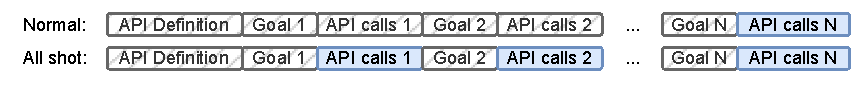
\includegraphics[width=0.85\textwidth]{plots/all_shot.pdf}
\label{fig:all_shot}
\end{figure}
To construct the training samples, we concatenate API documents and multiple pairs of goal and API calls as one input sequence to the LLMs. We use an all-shot loss formulation illustrated in~\Cref{fig:all_shot} which learns to generate the API calls for every goal in a sequence.
We use this loss formulation because it empirically delivers better success rate, especially when using in-context demonstrations, than the conventional loss which only backpropagates the loss associated with the API calls for the last goal.

\subsection{Training details}

We finetune each model on the same dataset created with the method described in Section \ref{sec:training_data_section} for $8$ epochs. We use a max sequence length of $2048$ without packing and mix the data from all the tasks into a single dataset with random shuffling. In each sample, all the goal-action pairs are from the same task. We report the validation accuracy on the best checkpoint. We use a batch size of 16 and a constant learning rate of $1e-5$ for each model and train on an internal cluster of 4 A100 GPU's, each with 80GB RAM.





\begin{table}[]
\caption{The detailed performance on the \snact~of models with different techniques applied. Mean(standard deviation) values are provided for each task. There exists some inevitable randomness, but it won't cange the results by too much.}
\label{tab:baselines_over_techniques}
\begin{adjustbox}{max width=\textwidth}
\setlength{\tabcolsep}{2pt}
\begin{tabular}{@{}cccccccccc@{}}
\toprule
                                          & \textbf{Open}                           & \textbf{The Cat}                    & \textbf{Home}        & \textbf{Trip}        & \textbf{Google}      &                                        & \multicolumn{2}{c}{\textbf{WebShop}}        &                                     \\
\multirow{-2}{*}{\textbf{Task}}           & {\color[HTML]{1F1F1F} \textbf{Weather}} & {\color[HTML]{1F1F1F} \textbf{API}} & \textbf{Search}      & \textbf{Booking}     & \textbf{Sheets}      & \multirow{-2}{*}{\textbf{VirtualHome}} & \textbf{Long}        & \textbf{Short}       & \multirow{-2}{*}{\textbf{Tabletop}} \\
\midrule
\textit{\textbf{Zero-shot Baseline}}          & \multicolumn{1}{l}{} & \multicolumn{1}{l}{} & \multicolumn{1}{l}{} & \multicolumn{1}{l}{} & \multicolumn{1}{l}{} & \multicolumn{1}{l}{}  & \multicolumn{1}{l}{} & \multicolumn{1}{l}{} & \multicolumn{1}{l}{} \\
gpt4                                          & 81.3(1.7)            & 97.4(0.3)            & 76.6(1.1)            & 91.5(0.5)            & 5.7(0.0)             & 40.8(0.6) / 8.0(0.2)  & 0.0(0.0)             & -                    & -                    \\
llama-30b                                     & 39.0(0.0)            & 49.0(0.0)            & 0.0(0.0)             & 0.0(0.0)             & 0.0(0.0)             & 78.0(0.0) / 0.3(0.0)  & 0.0(0.0)             & -                    & -                    \\
starcoder                                     & 32.0(0.0)            & 71.0(0.0)            & 7.0(0.0)             & 13.3(0.0)            & 5.9(1.1)             & 22.0(0.0) / 3.7(0.0)  & 0.0(0.0)             & -                    & -                    \\
codegen-16B-mono                              & 7.0(0.0)             & 78.0(0.0)            & 0.0(0.0)             & 0.0(0.0)             & 1.4(0.0)             & 4.0(0.0) / 1.0(0.0)   & 0.0(0.0)             & -                    & -                    \\
\cmidrule(lr){1-10}
\textit{\textbf{Sys. Prompt}}                 & \multicolumn{1}{l}{} & \multicolumn{1}{l}{} & \multicolumn{1}{l}{} & \multicolumn{1}{l}{} & \multicolumn{1}{l}{} & \multicolumn{1}{l}{}  & \multicolumn{1}{l}{} & \multicolumn{1}{l}{} & \multicolumn{1}{l}{} \\
gpt4                                          & 78.4(0.3)            & 94.2(0.8)            & 72.7(2.0)            & 89.6(0.9)            & 28.6(0.0)            & 42.8(0.6) / 8.6(0.1)  & 0.0(0.0)             & -                    & -                    \\
llama-30b                                     & 50.0(0.0)            & 88.0(0.0)            & 0.0(0.0)             & 0.0(0.0)             & 11.4(0.0)            & 24.0(0.0) / 2.5(0.0)  & 0.0(0.0)             & -                    & -                    \\
starcoder                                     & 71.0(0.0)            & 91.0(0.0)            & 2.0(0.0)             & 7.5(0.0)             & 15.9(0.2)            & 26.0(0.0) / 4.9(0.0)  & 0.0(0.0)             & -                    & -                    \\
codegen-16B-mono                              & 32.0(0.0)            & 69.0(0.0)            & 0.0(0.0)             & 0.0(0.0)             & 7.1(0.0)             & 5.0(0.0) / 1.6(0.0)   & 0.0(0.0)             & -                    & -                    \\
\cmidrule(lr){1-10}
\textit{\textbf{3-shot}}                      & \multicolumn{1}{l}{} & \multicolumn{1}{l}{} & \multicolumn{1}{l}{} & \multicolumn{1}{l}{} & \multicolumn{1}{l}{} & \multicolumn{1}{l}{}  & \multicolumn{1}{l}{} & \multicolumn{1}{l}{} & \multicolumn{1}{l}{} \\
gpt4                                          & 93.0(0.0)             & 96.0(0.0)             & 97.0(0.0)             & 96.7(0.0)             & 62.9(0.0)            & 23.0(0.0) / 23.5(0.0)   & 0.0(0.0)             & 0.0(0.0)             & 81.0(0.0)             \\
llama-30b                                     & 78.0(0.0)            & 84.0(0.0)            & 66.0(0.0)            & 45.0(0.0)            & 37.1(0.0)            & 27.0(0.0) / 21.7(0.0) & 0.0(0.0)             & 30.6(0.0)            & 34.3(0.0)            \\
starcoder                                     & 91.0(0.0)            & 84.0(0.0)            & 82.0(0.0)            & 51.7(0.0)            & 48.0(1.1)            & 23.0(0.0) / 19.4(0.0) & 2.6(0.0)             & 0.0(0.0)             & 21.9(0.0)            \\
codegen-16B-mono                              & 63.7(0.5)            & 72.0(0.0)            & 52.0(0.0)            & 28.3(0.0)            & 31.5(0.5)            & 28.0(0.0) / 15.7(0.0) & 1.5(0.0)             & 6.6(0.0)             & 15.2(0.0)            \\
\cmidrule(lr){1-10}
\textit{\textbf{Alignment}}                   & \multicolumn{1}{l}{} & \multicolumn{1}{l}{} & \multicolumn{1}{l}{} & \multicolumn{1}{l}{} & \multicolumn{1}{l}{} & \multicolumn{1}{l}{}  & \multicolumn{1}{l}{} & \multicolumn{1}{l}{} & \multicolumn{1}{l}{} \\
llama-30b                                     & 100.0(0.0)           & 94.0(0.0)            & 85.0(0.0)            & 87.5(0.0)            & 4.3(0.0)             & 14.0(0.0) / 10.6(0.0) & 20.8(0.0)            & -                    & -                    \\
starcoder                                     & 95.0(0.0)            & 98.0(0.0)            & 78.0(0.0)            & 85.0(0.0)            & 10.0(0.0)            & 28.0(0.0) / 13.4(0.0) & 0.0(0.0)             & -                    & -                    \\
codegen-16B-mono                              & 99.0(0.0)            & 95.8(0.6)            & 78.0(0.0)            & 73.3(0.0)            & 10.0(0.0)            & 10.0(0.0) / 11.5(0.0) & 30.3(0.0)            & -                    & -                    \\
\cmidrule(lr){1-10}
\textit{\textbf{Sys. Prompt + 3-shot}}        & \multicolumn{1}{l}{} & \multicolumn{1}{l}{} & \multicolumn{1}{l}{} & \multicolumn{1}{l}{} & \multicolumn{1}{l}{} & \multicolumn{1}{l}{}  & \multicolumn{1}{l}{} & \multicolumn{1}{l}{} & -                    \\
gpt4                                          & 99.0(0.0)            & 98.0(0.0)            & 98.0(0.0)            & 99.2(0.0)            & 68.6(0.0)            & 29.0(0.0) / 21.7(0.0) & 0.0(0.0)             & 0.0(0.0)             & 83.8(0.0)            \\
llama-30b                                     & 66.0(0.0)            & 82.0(0.0)            & 63.0(0.0)            & 45.8(0.0)            & 27.1(0.0)            & 34.0(0.0) / 20.5(0.0) & 0.0(0.0)             & 0.0(0.0)             & 34.6(0.2)            \\
starcoder                                     & 92.0(0.0)            & 91.0(0.0)            & 73.0(0.0)            & 54.2(0.0)            & 50.0(0.2)            & 28.0(0.0) / 15.0(0.0) & 0.0(0.0)             & 0.0(0.0)             & 23.4(0.3)            \\
codegen-16B-mono                              & 64.2(0.3)            & 70.0(0.0)            & 45.0(0.0)            & 22.5(0.0)            & 28.6(0.9)            & 27.0(0.0) / 15.7(0.0) & 0.0(0.0)             & 0.0(0.0)             & 14.6(0.2)            \\
\cmidrule(lr){1-10}
\textit{\textbf{Sys. Prompt + Alignment}}     &                      & \multicolumn{1}{l}{} & \multicolumn{1}{l}{} & \multicolumn{1}{l}{} & \multicolumn{1}{l}{} & \multicolumn{1}{l}{}  & \multicolumn{1}{l}{} & \multicolumn{1}{l}{} & \multicolumn{1}{l}{} \\
llama-30b                                     & 100.0(0.0)           & 94.0(0.0)            & 79.0(0.0)            & 80.8(0.0)            & 5.7(0.0)             & 10.0(0.0) / 10.3(0.0) & 0.6(0.0)             & -                    & -                    \\
starcoder                                     & 98.7(0.2)            & 97.0(0.0)            & 79.0(0.0)            & 84.2(0.0)            & 10.0(0.0)            & 18.0(0.0) / 10.3(0.0) & 0.0(0.0)             & -                    & -                    \\
codegen-16B-mono                              & 99.0(0.0)            & 96.0(0.0)            & 77.0(0.0)            & 75.8(0.0)            & 8.6(0.0)             & 7.0(0.0) / 10.0(0.0)  & 25.7(0.0)            & -                    & -                    \\
\cmidrule(lr){1-10}
\textit{\textbf{3-shot + Alignment}}          & \multicolumn{1}{l}{} & \multicolumn{1}{l}{} & \multicolumn{1}{l}{} & \multicolumn{1}{l}{} & \multicolumn{1}{l}{} & \multicolumn{1}{l}{}  & \multicolumn{1}{l}{} & \multicolumn{1}{l}{} & \multicolumn{1}{l}{} \\
llama-30b                                     & 100.0(0.0)           & 94.0(0.0)            & 88.0(0.0)            & 89.2(0.0)            & 4.3(0.0)             & 20.0(0.0) / 26.3(0.0) & 19.5(0.0)            & 15.1(0.0)            & 6.9(0.2)             \\
starcoder                                     & 100.0(0.0)           & 96.0(0.0)            & 91.0(0.0)            & 84.2(0.0)            & 15.7(0.0)            & 48.0(0.0) / 21.3(0.0) & 0.0(0.0)             & 0.0(0.0)             & 13.9(0.3)            \\
codegen-16B-mono                              & 99.0(0.0)            & 97.9(0.2)            & 80.0(0.0)            & 77.5(0.0)            & 16.4(0.9)            & 38.0(0.0) / 18.6(0.0) & 6.5(0.0)             & 17.5(0.0)            & 16.2(0.0)            \\
\cmidrule(lr){1-10}
\textit{\textbf{Prompt + 3-shot + Alignment}} & \multicolumn{1}{l}{} & \multicolumn{1}{l}{} & \multicolumn{1}{l}{} & \multicolumn{1}{l}{} & \multicolumn{1}{l}{} & \multicolumn{1}{l}{}  & \multicolumn{1}{l}{} & \multicolumn{1}{l}{} & \multicolumn{1}{l}{} \\
llama-30b                                     & 100.0(0.0)           & 94.0(0.0)            & 87.0(0.0)            & 85.8(0.0)            & 2.9(0.0)             & 16.0(0.0) / 24.3(0.0) & 0.0(0.0)             & 0.0(0.0)             & 7.5(0.1)             \\
starcoder                                     & 99.0(0.0)            & 97.0(0.0)            & 83.0(0.0)            & 80.8(0.0)            & 21.2(0.3)            & 31.0(0.0) / 18.4(0.0) & 0.0(0.0)             & 0.0(0.0)             & 13.9(0.3)            \\
codegen-16B-mono                              & 97.7(0.2)            & 99.0(0.0)            & 82.0(0.0)            & 77.5(0.0)            & 19.8(0.3)            & 29.0(0.0) / 17.2(0.0) & 0.0(0.0)             & 3.5(0.0)             & 16.2(0.0)                    \\
\bottomrule
\end{tabular}
\end{adjustbox}
\end{table}



% \begin{table}[]
% \caption{The detailed performance on the \snact~of models with different techniques applied.}
% \label{tab:baselines_over_techniques}
% \begin{adjustbox}{max width=\textwidth}
% \setlength{\tabcolsep}{3pt}
% \begin{tabular}{@{}cccccccccc@{}}
% \toprule
%                                           & \textbf{Open}                           & \textbf{The Cat}                    & \textbf{Home}        & \textbf{Trip}        & \textbf{Google}      &                                        & \multicolumn{2}{c}{\textbf{WebShop}}        &                                     \\
% \multirow{-2}{*}{\textbf{Task}}           & {\color[HTML]{1F1F1F} \textbf{Weather}} & {\color[HTML]{1F1F1F} \textbf{API}} & \textbf{Search}      & \textbf{Booking}     & \textbf{Sheets}      & \multirow{-2}{*}{\textbf{VirtualHome}} & \textbf{Long}        & \textbf{Short}       & \multirow{-2}{*}{\textbf{Tabletop}} \\
% \midrule
% \textit{\textbf{Zero-shot Baseline}}      & \multicolumn{1}{l}{}                    & \multicolumn{1}{l}{}                & \multicolumn{1}{l}{} & \multicolumn{1}{l}{} & \multicolumn{1}{l}{} & \multicolumn{1}{l}{}                   & \multicolumn{1}{l}{} & \multicolumn{1}{l}{} & \multicolumn{1}{l}{}                \\
% gpt4                                      & 70.0                                    & 80.0                                & 70.0                 & 45.0                 & 5.7                  & 29.0 / 9.5                             & 0.0                  & -                    & -                                   \\
% llama-30b                                 & 6.0                                     & 5.0                                 & 0.0                  & 0.0                  & 0.0                  & 3.0 / 0.1                              & 0.0                  & -                    & -                                   \\
% codegen-16B-mono                          & 12.0                                    & 47.0                                & 0.0                  & 0.0                  & 0.0                  & 0.0 / 0.6                              & 0.0                  & -                    & -                                   \\
% \midrule
% \textit{\textbf{Sys. Prompt}}             & \multicolumn{1}{l}{}                    & \multicolumn{1}{l}{}                & \multicolumn{1}{l}{} & \multicolumn{1}{l}{} & \multicolumn{1}{l}{} & \multicolumn{1}{l}{}                   & \multicolumn{1}{l}{} & \multicolumn{1}{l}{} & \multicolumn{1}{l}{}                \\
% gpt4                                      & 81.0                                    & 96.0                                & 74.0                 & 92.5                 & 28.6                 & 49.0 / 9.3                             & 0.0                  & -                    & -                                   \\
% llama-30b                                 & 52.0                                    & 87.0                                & 0.0                  & 0.0                  & 10.0                 & 24.0 / 2.5                             & 0.0                  & -                    & -                                   \\
% codegen-16B-mono                          & 32.0                                    & 72.0                                & 0.0                  & 0.0                  & 7.1                  & 5.0 / 1.5                              & 0.0                  & -                    & -                                   \\
% \cmidrule(lr){1-10}
% \textit{\textbf{3-shot}}                  & \multicolumn{1}{l}{}                    & \multicolumn{1}{l}{}                & \multicolumn{1}{l}{} & \multicolumn{1}{l}{} & \multicolumn{1}{l}{} & \multicolumn{1}{l}{}                   & \multicolumn{1}{l}{} & \multicolumn{1}{l}{} & \multicolumn{1}{l}{}                \\
% gpt4                                      & 93.0                                    & 96.0                                & 97.0                 & 96.7                 & 62.9                 & 23.0 / 23.5                            & 0.0                  & 0.0                  & 81.0                                \\
% llama-30b                                 & 80.0                                    & 84.0                                & 65.0                 & 45.8                 & 37.1                 & 25.0 / 21.5                            & 0.0                  & 31.4                 & 34.3                                \\
% codegen-16B-mono                          & 65.0                                    & 72.0                                & 52.0                 & 22.5                 & 38.6                 & 26.0 / 15.5                            & 0.0                  & 5.7                  & 14.3                                \\
% \cmidrule(lr){1-10}
% \textit{\textbf{Alignment}}               & \multicolumn{1}{l}{}                    & \multicolumn{1}{l}{}                & \multicolumn{1}{l}{} & \multicolumn{1}{l}{} & \multicolumn{1}{l}{} & \multicolumn{1}{l}{}                   & \multicolumn{1}{l}{} & \multicolumn{1}{l}{} & \multicolumn{1}{l}{}                \\
% llama-30b & 100.0 & 94.0 & 85.0 & 87.5 & 4.3 & 12.0 / 12.9 & 20.8 & - & - \\
% codegen-16B-mono                          & 99.0                                    & 95.0                                & 78.0                 & 74.2                 & 8.6                  & 14.0 / 14.6                            & 32.0                 & -                    & -                                   \\
% \midrule
% \textit{\textbf{Sys. Prompt + 3-shot}}    & \multicolumn{1}{l}{}                    & \multicolumn{1}{l}{}                & \multicolumn{1}{l}{} & \multicolumn{1}{l}{} & \multicolumn{1}{l}{} & \multicolumn{1}{l}{}                   & \multicolumn{1}{l}{} & \multicolumn{1}{l}{} & \multicolumn{1}{l}{}                \\
% gpt4                                      & 99.0                                    & 98.0                                & 98.0                 & 99.2                 & 68.6                 & 29.0 / 21.7                            & 0.0                  & 0.0                  & 83.8                                \\
% llama-30b                                 & 83.0                                    & 81.0                                & 63.0                 & 45.8                 & 27.1                 & 31.0 / 21.5                            & 0.0                  & 0.0                  & 34.3                                \\
% codegen-16B-mono                          & 63.0                                    & 67.0                                & 45.0                 & 27.5                 & 28.6                 & 22.0 / 15.3                            & 0.0                  & 0.0                  & 14.3                                \\
% \cmidrule(lr){1-10}
% \textit{\textbf{Sys. Prompt + Alignment}} & \multicolumn{1}{l}{}                    & \multicolumn{1}{l}{}                & \multicolumn{1}{l}{} & \multicolumn{1}{l}{} & \multicolumn{1}{l}{} & \multicolumn{1}{l}{}                   & \multicolumn{1}{l}{} & \multicolumn{1}{l}{} & \multicolumn{1}{l}{}                \\
% llama-30b & 100.0 & 94.0 & 78.0 & 80.8 & 7.1 & 9.0 / 10.5 & 0.0 & - & -\\
% codegen-16B-mono                          & 99.0                                    & 96.0                                & 77.0                 & 75.8                 & 8.6                  & 6.0 / 10.0                             & 27.3                 & -                    & -                                   \\
% \cmidrule(lr){1-10}
% \textit{\textbf{3-shot + Alignment}}      & \multicolumn{1}{l}{}                    & \multicolumn{1}{l}{}                & \multicolumn{1}{l}{} & \multicolumn{1}{l}{} & \multicolumn{1}{l}{} & \multicolumn{1}{l}{}                   & \multicolumn{1}{l}{} & \multicolumn{1}{l}{} & \multicolumn{1}{l}{}                \\
% llama-30b & 100.0 & 94.0 & 88.0 & 89.2 & 4.3 & 16.0 / 26.1 & 18.8 & 16.2 & 6.7 \\
% codegen-16B-mono                          & 98.0                                    & 98.0                                & 81.0                 & 75.8                 & 18.6                 & 39.0 / 19.0                            & 5.5                  & 22.7                 & 16.2                                \\
% \midrule
% \textit{\textbf{Prompt + 3-shot + Alignment}}      & \multicolumn{1}{l}{}                    & \multicolumn{1}{l}{}                & \multicolumn{1}{l}{} & \multicolumn{1}{l}{} & \multicolumn{1}{l}{} & \multicolumn{1}{l}{}                   & \multicolumn{1}{l}{} & \multicolumn{1}{l}{} & \multicolumn{1}{l}{}                \\
% llama-30b & 100.0 & 95.0 & 86.0 & 85.8 & 2.9 & 15.0 / 26.4 & 0.0 & 0.0 & 7.6 \\
% codegen-16B-mono                          & 99.0                                    & 99.0                                & 83.0                 & 76.7                 & 18.6                 & 37.0 / 19.3                            & 0.0                  & 13.2                 & 16.2                               \\
% \bottomrule
% \end{tabular}
% \end{adjustbox}
% \end{table}
\subsection{Extended results for \Cref{sec:experiments}}
We list out the detailed results of \Cref{sec:experiments} in \Cref{tab:baselines_over_techniques}, where we report the model performance on all the possible combinations of the three proposed techniques. The main observations are all covered in \Cref{sec:experiments}. We run each job 3 times, and report the mean and standard deviation of the main metrics. Their are some inevitable randomness happens in API or example retrieval, public API services and the environment provided in Webshop and Tabletop. Even though randoness exists, we observe that they barely change the final results. Thus, we only report the mean value everywhere else in the paper.



